% Chapter 4

\chapter{Results}

\label{Chapter4}

We begin our discussion of the results with preliminary analysis of the data. Here we seek to understand some of the overarching patterns in listening habits and how these look at an individual level. After this we present a summary of our results followed by a discussion of the performance of each individual method.

\section{Preliminary analysis}

\subsection{Daily play patterns}

By grouping track plays into 30 min intervals and aggregating by periods within a day, we see a clear daily pattern with music listening hitting a peak at around 5pm and a trough at around 6am (fig. \ref{3a}).

\begin{figure}[h!]
	\centering
	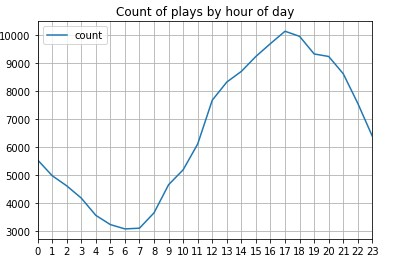
\includegraphics[width=7cm, keepaspectratio,]{fig004.jpg}
	\caption{5-5.30pm is peak listening time}
	\label{3a}
\end{figure} 

Zooming out to view the pattern across an entire week in fig. \ref{3b}, we see that the daily pattern occurs across every day of the week with weekends having a lower total number of plays.

\begin{figure}[h!]
	\centering
	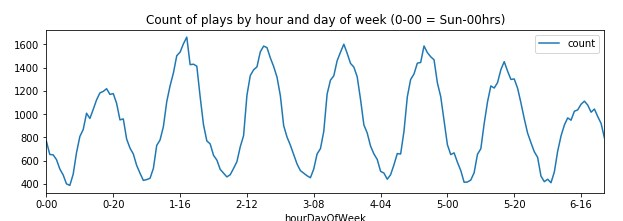
\includegraphics[width=12cm, keepaspectratio,]{fig005.jpg}
	\caption{Most popular times to listen to music across all users}
	\label{3b}
\end{figure} 

At an aggregate level therefore one can get good accuracy by simply anticipating music demand to peak at 5pm. However if we select two users at random (fig. \ref{3c}), we see that these daily patters are not as strongly discernible. As we see later this is likely impacting the Bayesian Inference model as it begins with using the population distribution as the prior. 

\begin{figure}[h!]
	\centering
	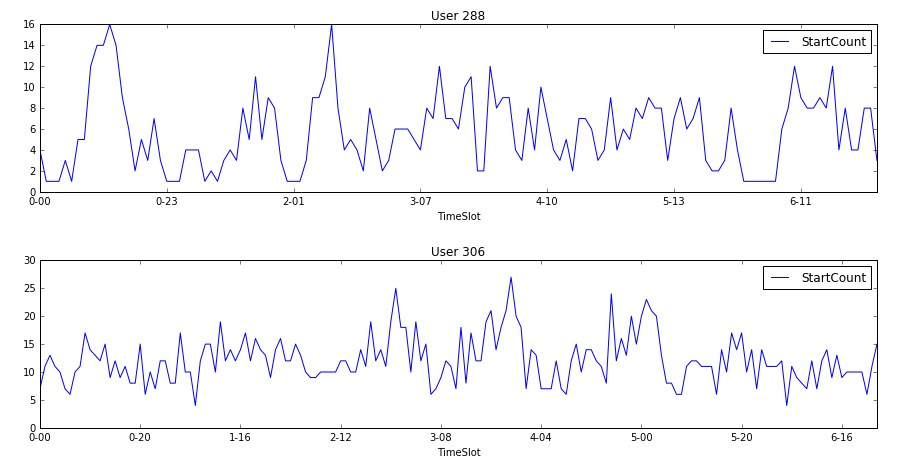
\includegraphics[width=12cm, keepaspectratio,]{fig006.jpg}
	\caption{Most popular times to listen to music by individual user}
	\label{3c}
\end{figure} 

\subsection{Outlier analysis}

The dataset contains a timestamp associated with each user. This does not necessarily mean the user played a song in its entirety. Analysis shows plenty of cases where the interval time between tracks was a few seconds suggesting the user skipped tracks. 

\begin{figure}[h!]
	\centering
	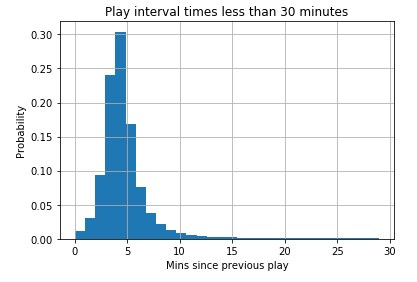
\includegraphics[width=8cm, keepaspectratio,]{fig003.jpg}
	\caption{}
	\label{3d}
\end{figure} 

Fig. \ref{3d} shows a frequency plot of intervals. Intervals beyond 30 minutes continue the exponential decrease and are not shown. We see that while the mode is on par with a typical song length, there is a significant number of plays that lasted under 5 minutes. For our purposes these are include as evidence that the user was interested in playing music at time $t$ and therefore treated as a Play event.

Further analysis showed one user in particular with very high amount of plays, with very low durations, suggesting it was likely to have been generated by a bot, possibly a LastFM test. This was excluded from the dataset.

Fig. \ref{fig25} shows the histogram for plays greater than a day. 
\begin{figure}[h!]
	\centering
	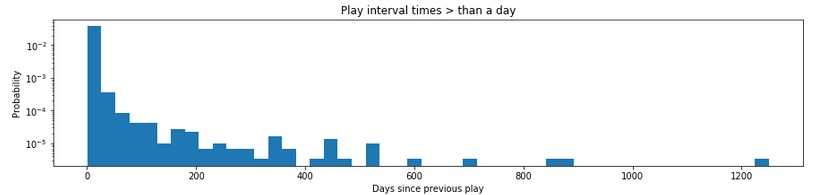
\includegraphics[width=13cm, keepaspectratio,]{fig025.jpg}
	\caption{}
	\label{fig25}
\end{figure} 

As one would expect the probability of someone playing music decreases the longer in time they go without playing music. For any music recommender system being able to predict whether a user is likely to listen to music in 1 day, 200 days, or 1200 days, would allow for different strategies for user retention.

\subsection{Time-series analysis}

Here we examine our data once it has been transformed into a binary sequence of play events (1) and non-play events(0). We seek to understand better how an optimizer may perform based on traits of the data.

We begin with assessing how well our baseline model may perform. Fig. \ref{fig12} shows that the 76\% of Plays, also had a play in $t-1$. However this rule also captures 2.2\% of non-plays events.

\begin{figure}[h!]
	\centering
	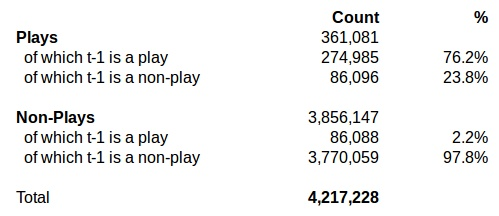
\includegraphics[width=7cm, keepaspectratio,]{fig012.jpg}
	\caption{}
	\label{fig12}
\end{figure} 

The 23.8\% of Plays that did not have a play in the prior period are harder to predict, yet are of more interest as they represent the beginning of a listening period. 

Given the daily patterns we have seen, it might be reasonable to assume that $t-24hrs$ may help us to determine the start of an session. However analysis shows that in only 34\% of play events was there also a play event in 24 hours prior.

What both of these results tell us is that fairly high precision score of around 76\% ought ot be possible purely based on $t-1$ but going above this will be a lot harder.

\section{Main results} % Methodology

\subsection{Summary}

Fig. \ref{fig13b} shows the results from across all experiments after 5-fold cross validation.

\begin{figure}[h!]
	\centering
	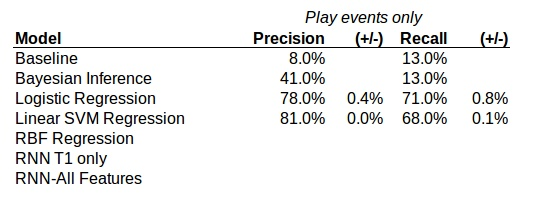
\includegraphics[width=8cm, keepaspectratio,]{fig013b.jpg}
	\caption{Summary of results}
	\label{fig13b}
\end{figure}  

We see that none of the models score better than the Baseline model. The logistic regression model is able to match the Baseline model once we restrict the input to $t-1$. 

It may be that $t = t-1$ is the only pattern that is consistently important across users, with all other time-lags having too much variance across users for them to be useful.

In a similar vein, the Bayesian Inference model performed poorly on both measures, suggesting that that the difference between the population and what is observed at an individual level differs too much for the prior probability to be accurate for any one individual user, something we saw some indications for in our preliminary analysis. 

Our remaining models exhibit the the tension between good accuracy and good recall, with only the RBF SVM model demonstrating the ability to reach a balance score across both. The Logistic regression and RNN models perform below average on precision but well on recall, while the Linear SVM model scores better on precision. We will discuss each one model in turn next.
 
\section{Beta-Binomial Model}

We outline here how the model was derived in order to aid understanding of its performance. 

We can plot the prior probability for any given time period, as shown in fig. \ref{fig10c}.

\begin{figure}[h!]
	\centering
	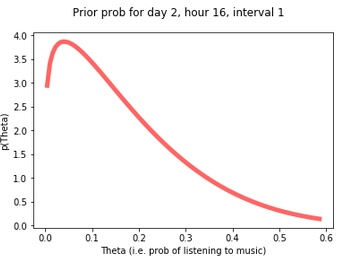
\includegraphics[width=5cm, keepaspectratio,]{fig010c.jpg}
	\caption{}
	\label{fig10c}
\end{figure} 

Here we see that $\theta$, which represents the prior probability of listening to music in the specified timeslot, is likely to be less than 0.1. Notice that this timeslot is for hour 17 (i.e. 5pm) which, from our preliminary analysis, we  know is the peak listening time at an aggregate level. The fact that the probability is so low for this timeslot would likely be due to the presence of lots of 5pm periods in which music was not listened to at the individual user level. For instance - if our dataset contains large gaps between weeks in which music was listened to. 

For our posterior function, the threshold at which we determine a play event was determined by comparing the false positive rates with the true positive rates using a ROC curve (fig. \ref{fig10d}). From this 0.4 was selected as the optimal threshold at which to determine a Play event across all users.

\begin{figure}[h!]
	\centering
	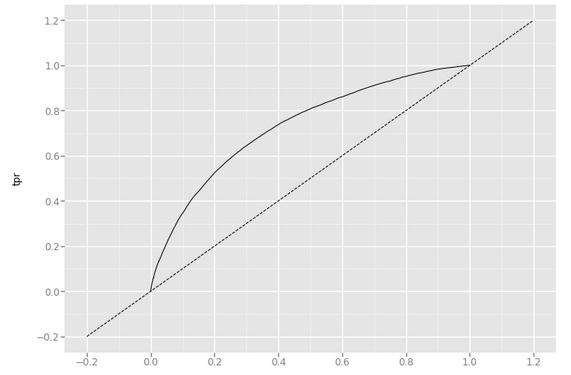
\includegraphics[width=5cm, keepaspectratio,]{fig010d.jpg}
	\caption{ROC curve showing 0.4 as the optimal threshold}
	\label{fig10d}
\end{figure} 

The results from the model are shown in table \ref{tabA}. We see that the recall and precision of play events (as denoted by 1) is very low. Clearly the approach of building up a weekly profile based on the population then updating it with individual observations is not very effective. This does not however rule some other form of Bayesian modelling such as Bayesian Logistic Regression.

\begin{table}[h!]
	\centering
	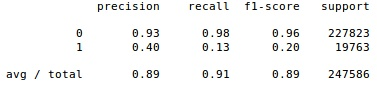
\includegraphics[width=7cm, keepaspectratio,]{fig010e.jpg}
	\caption{Beta-Binomial Model Results}
	\label{tabA}
\end{table} 

\section{Logistic regression analysis}

For logistic regression we are able to examine the coefficients to understand how the model is making use of the input data.

\begin{table}[h!]
	\centering
	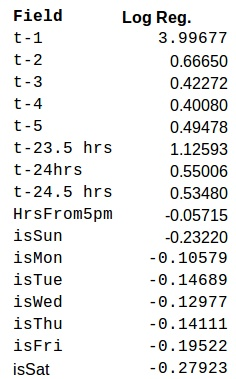
\includegraphics[width=4cm, keepaspectratio,]{fig014.jpg}
	\caption{}
	\label{tabB}
\end{table} 

Table \ref{tabB} shows that $t-1$ was by far the most important feature and its importance crowds out the other features. Interestingly $t-23.5$ is the second strongest time-lag and more significant than t-24hrs. As t-23.5 would be 24 hours prior to $t-1$, it suggests that having a consistent $t-1$ is more important than simply knowing what $t$ was 24 hours prior; which we know from our preliminary analysis is not very effective anyway.

The non-time lag features seem to have very little effect. We see this in the forward stepwise regression chart in fig. \ref{fig16} which shows that the inclusion of additional features barely impacts the results.

\begin{figure}[h!]
	\centering
	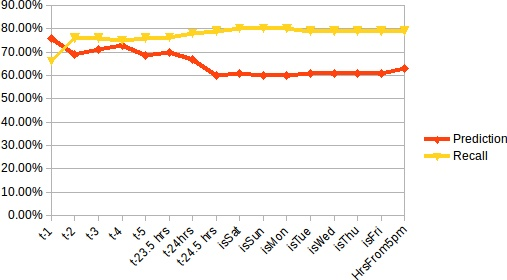
\includegraphics[width=7cm, keepaspectratio,]{fig016.jpg}
	\caption{Stepwise regression, adding in fields from left to right}
	\label{fig16}
\end{figure} 

\section{SVM analysis}

That the Linear SVM performs well on precision but not recall may be due to it ignoring probabilities that fall within the margin of the decision boundary during optimization, such as the start of a play sequence or ad-hoc plays by a user that do not fit their regular listening pattern. Hence the model is more likely to only predict a play event when the probability is sufficiently high.

The RBF model on the other hand performs well on both metrics. Note that the RBF classification was restricted to 100k rows of training data as it was found the computational cost of 500k rows was too high. 

In order to determine optimal $gamma$ and C values, a grid search was carried out with precision and recall of the test dataset plotted on a heat map. In order to get through the many iterations of the data, the input data was reduced to 30,000 training samples. Fig \ref{fig17b} shows the final heat map, after multiple iterations to home in on the optimal values, with precision on the left and recall on the right. The optimal values are deemed to be 0.6 for C and 0.76 for Gamma, although as the charts show there is some scope for movement around those values.

\begin{figure}[h!]
	\centering
	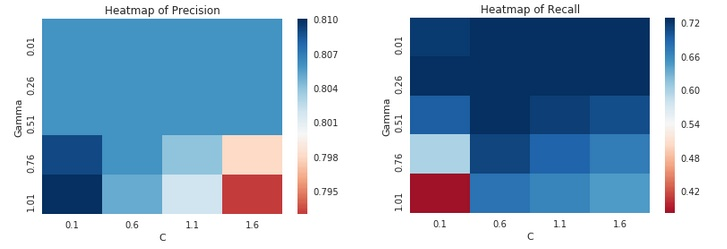
\includegraphics[width=8cm, keepaspectratio,]{fig017b.jpg}
	\caption{Heatmap of hyper-parameter search. Dark blue shade = better precision and recall}
	\label{fig17b}
\end{figure} 

The final results for the RBF model (precision of 77\%, recall of 76\%) was about the same when only $t-1$ was provided as an input, suggesting the RBF model is likely approximating to the $t=t-1$ rule used in the baseline model.

Finally, while we managed to get as high as 100,000 rows of our training in our training, the computational complexity of the RBF kernel meant it was not practical to go any higher thereby limiting the scalability of this approach and our ability to potentially obtain higher scores than what we already had.

\newpage

\section{RNN-LSTM analysis}

The RNN model had a large number of hyper-parameters to search through resulting in significantly more time required to train than the other models. Fig \ref{fig20} shows details of a few of these runs, including the model that gave the best set of results (run num. 4). Key differences between the runs are shaded in grey.

\begin{figure}[h!]
	\centering
	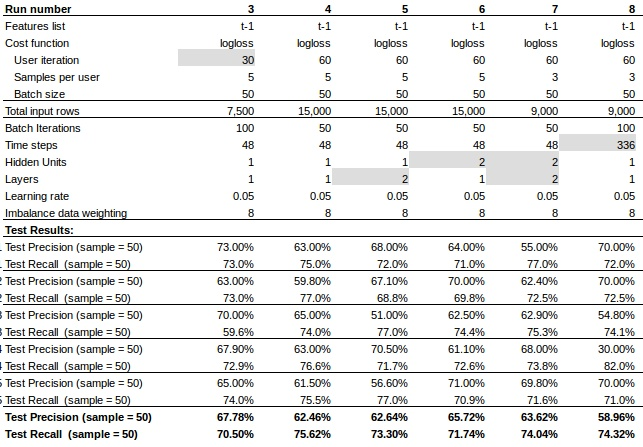
\includegraphics[width=12cm, keepaspectratio,]{fig020.jpg}
	\caption{Example of hyper-parameter search. Key settings shaded.}
	\label{fig20}
\end{figure} 


In total 50+ experiments were performed with different hyper-parameter settings. The following observations were made based on the results of all experiments.

\subsubsection{Early stopping}

Continued training of models eventually led to performance decrease, with predictions becoming either all play events or all non-play events depending on the weighting used. Possible measures to counteract this may be to use drop-outs, a form of regularization in neural networks. However this was not investigated. Instead models were trained up-to around 15,000 rows of data.

\subsubsection{More layers or units did not improve performance}

Moving up from 1 hidden unit and 1 hidden layer did not result in performance improvement, and performance started to drop if it increased too high (10 units or 3+ layers). It appears that this was due to the model over-fitting the data.
 
\subsubsection{The sample weighting was critical}

The amount of weighting required to deal with the data imbalance varies depending on how many rows of training data there are, and the level of imbalance. In our case 8 was found to be the level at which precision and recall remained high across a training set of 15,000 rows. Lower than this and all predictions soon converge to non-play events; higher than this they all become play events (and hence low precision, high recall).

\subsubsection{Going beyond a 24hour timestep did not improve performance}

Moving beyond a time-step of 48 (i.e. 24 hours) to 336 (1 week) or more led to a decrease in performance. This matches what we saw in the logistic regression model where periods beyond the 24 hour period had little impact in predicting outcome.

\section{Summary}

We found that the Linear SVM model achieves the highest precision, while the logistic regression and baseline models achieved the highest recall. Overall across both metrics, our baseline model performs the best. Furthermore from our examination of the coefficients and experiments with the RNN model, it did not appear that time-lags beyond 24 hours were a useful predictor. Indeed logistic regression performed best, and on-par with the baseline, when $t-1$ was the only input feature. These results suggests that additional features make it harder for the models to attribute the right level of importance to $t-1$. 

This may be an issue with the framing of the question and/or the nature of the dataset. As an addendum to our initial research, a quick analysis was performed on first play event data only. This dataset was constructed by removing all rows where there was a play event in periods $t-1$ to $t-5$, leaving behind rows where the user had not listened to music in the past 2.5 hours. We were interested in seeing how are our models performed without any tuning.

We found that all models performed poorly including the baseline (as would be expected), with precision and recall both at 0\% for all but the logistic regression model which had a precision of 0.7\% and a recall of 0.3\%. 

From a scalability perspective both the logistic model and linear SVM performed well on 500k rows of training data, RBF SVM was capped at 100k rows, and the RNN around 15-20k rows due to much more hyper-parameter testing. Using the logistic model as a guideline was also found to be helpful in determining parameters for the RNN. 